% vim: set spelllang=en :

\documentclass[10pt]{article}

\usepackage{amsmath, amssymb, amsfonts, amsthm} 
\usepackage{upgreek} 
\usepackage{amsthm} 
\usepackage{fullpage}
\usepackage{graphicx}
\usepackage{cancel}
\usepackage{wrapfig}
\usepackage{subfigure}
\usepackage{mathrsfs}
\usepackage{outlines}
\usepackage[font={sf,it}, labelfont={sf,bf}, labelsep=space, belowskip=5pt]{caption}
\usepackage{hyperref}
\usepackage{titling}
\usepackage{xifthen}
\usepackage{color}
\usepackage{fancyhdr}
\usepackage[title]{appendix}
\usepackage{float}
\usepackage{enumitem}

\usepackage{bm}
\usepackage{minted}
\usepackage{xcolor}

\pagestyle{fancy}
\headheight 24pt
\headsep    12pt
\lhead{\documenttitle}
\rhead{\today}
\fancyfoot[C]{}
\lfoot{}
\rfoot{\thepage}
\renewcommand{\headrulewidth}{0.4pt}
\renewcommand\footrulewidth{0.4pt}
\newcommand{\documenttitle}{Assignment Solution}
\newcommand{\coursetitle}{SE2324: Mathematical Foundation of Computer Sciences(Spring 2021)}
\newcommand{\authorname}{Student Name, ID1001001001} % Your name and ID here

\makeatletter

\setlength{\droptitle}{-50pt}

\title{\documenttitle \vspace{1ex} \\ \Large \coursetitle \vspace{-1ex}}
\author{\authorname\vspace{-1ex}}


% BEGIN DOCUMENT
\begin{document}
\maketitle


%%%%%%%%%%%%%%%%%%%
\section{README}

... 

%%%%%%%%%%%%%%%%%%%
\section{Eigenvectors (40 points)}

\paragraph{Guitar String Vibrations} In this question, we will study vibrations on a string.
 
The Helmholtz equation is useful for modeling the standing wave vibrations on a guitar string:

\begin{equation}
    \label{eq:helmholtz}
    \frac{d^2}{dx^2} y(x) + k^2y(x)=0.
\end{equation}

In this equation, $x$ is the location along the string, $y$ is the perpendicular displacement, and $k > 0$ can be any positive real.
Our string has length 1, i.e. $x \in [0, 1]$.
Both ends of the string are clamped, with boundary conditions $y(0) = y(1) = 0$, which should simplify our problem.

\subparagraph{Analytical Spectral Properties of the Laplacian operator} (15 points)

Let C be the set of twice-differentiable real functions $f(x)$ for $x \in (0, 1)$. We can consider $C$ a vector space: 
for functions $f(x)$ and $g(x)$, their sum $h(x) = f(x) + g(x)$ is in this space, and so is any scalar multiple $h(x) = a f(x)$. 
We also define an inner product,

$$
\langle f, g\rangle=\int_{0}^{1} f(x) g(x) d x.
$$

The Laplacian operator is therefore a linear transformation $M$, which takes a function $f \in C$ as input and outputs its second derivative:

$$
M f=\frac{d^{2}}{d x^{2}} f
$$

\begin{enumerate}[label=2.\arabic*]
    \item (8 points) \label{q:eigenvector}
    Verify that functions of the form $\psi_{n}(x)=\sqrt{2} \sin (\pi n x)$,
    for positive integer $n$, are eigenvectors of the Laplacian with eigenvalue $\lambda_{n}=-n^{2} \pi^{2}$.
    (I.e. verify $M \psi_{n}(x)=\lambda_{n} \psi_{n}(x)$ )\par
    $M \psi_{n}(x)=\frac{d^{2}}{d x^{2}}\sqrt{2} \sin (\pi n x)=-\sqrt{2}\pi^2n^2\sin{\pi nx}$\par
    Also, $\lambda_{n} \psi_{n}(x)=-n^2\pi^2\sqrt{2} \sin (\pi n x)=-\sqrt{2}\pi^2n^2\sin{\pi nx}$\par
	So $M \psi_{n}(x)=\lambda_{n} \psi_{n}(x)$\par
    \item (8 points) \label{q:orthonormal-eigenvector}
    Verify that these eigenvectors $\left\{\psi_{n}\right\}$ are orthonormal, i.e.
\begin{equation}
    \int_{0}^{1} \psi_{n}(x) \psi_{m}(x) d x=
    \left\{\begin{array}{ll}
        1 & \text { if } n=m \\
        0 & \text { otherwise }
    \end{array}\right.
\end{equation}
Hint: Please prove the statements in Question \ref{q:eigenvector} and \ref{q:orthonormal-eigenvector} mathematically. You can use the trigonometric identity: $2\sin u \sin v = \cos (u-v) - \cos (u+v)$.\par
Proof:\par
If $m \neq n:$
\begin{equation}
\int_{0}^{1} \psi_{n}(x) \psi_{m}(x) d x=\int_{0}^{1} 2\sin{\pi nx}\sin{\pi mx} d x 
\end{equation}
\begin{equation}
= \int_{0}^{1}\cos{(n-m)\pi x}- \cos{(n+m)\pi x} d x=\frac{\sin{(n-m)\pi}}{(n-m)\pi} - \frac{\sin{(n+m)\pi}}{(n+m)\pi}=0
\end{equation}
if $m=n$:\par
\begin{equation}
\int_{0}^{1} \psi_{n}(x) \psi_{m}(x) d x=\int_{0}^{1} 2\sin^2{\pi nx} d x = \int_{0}^{1} 1-\cos{2\pi nx} d x =1
\end{equation}
Namely 
\begin{equation}
\int_{0}^{1} \psi_{n}(x) \psi_{m}(x) d x=
\left\{\begin{array}{ll}
1 & \text { if } n=m \\
0 & \text { otherwise }
\end{array}\right.
\end{equation}
So the eigenvectors are orthonormal.
\end{enumerate}

\subparagraph{Discrete Solutions}(30 points)

Similar to the previous assignment, 
we can discretize $y(x)$ over a grid of $N = 99$ interior values, with the first value $x_1 = 0.01$ and the last value $_{99} = 0.99$.
As before, $y(0) = y(1) = 0$. 
Denote the spacing as $h = \frac{1}{N+1}$.
For any function $f(x)$, we will use the notation $\vec{f}$ to denote $(f(x_1), f(x_2), ..., f(x_N))^T$

Given the discrete derivative of a function using central difference as

\begin{equation}
    f^{\prime}(x)=\frac{f\left(x+\frac{h}{2}\right)-f\left(x-\frac{h}{2}\right)}{h},
\end{equation}

we can get the discrete form of the Laplacian operator by applying this equation twice

\begin{equation}
\begin{aligned}
    f^{\prime\prime}(x)&=\frac{f^\prime\left(x+\frac{h}{2}\right)-f^\prime\left(x-\frac{h}{2}\right)}{h}\\
    &=\frac{
    \frac{f\left(x+h\right)-f\left(x\right)}{h}
    -\frac{f\left(x\right)-f\left(x-h\right)}{h}
    }{h}\\
    &=\frac{f\left(x+h\right)-2f\left(x\right)+f\left(x-h\right)}{h^2}
\end{aligned}
\end{equation}


With the $1 \mathrm{D}$ Laplacian matrix $A$ of dimension $N \times N$

\begin{equation}
A_{i j}=
    \left\{\begin{array}{ll}
        -2 & \text { if } i=j \\
        1 & \text { if }|i-j|=1 \\
        0 & \text { otherwise }
    \end{array}\right.
\end{equation}

we have $\overrightarrow{f^{\prime \prime}}=h^{-2} A \vec{f}$. 
We will now use $M$ to denote $h^{-2} A$.

\begin{enumerate}[label=2.\arabic*]
\setcounter{enumi}{2}

    \item (12 points) 
    Construct $M$ and $\vec{y}$ in Python for $y(x)=\psi_{1}(x)$ and verify that $\vec{y}$ satisfies the Helmholtz equation \ref{eq:helmholtz}.
    % plot $M \vec{y}$ and $-\pi^{2} \vec{y}$ separately, and verify that the plots are identical.
    % (Hint: It might be more convenient, for functions you will need later, to represent $M$ as a SymTridiagon Tridiagonal, or a full matrix, rather than a sparse matrix.)
   	\begin{figure}[H]
    	\centering
    	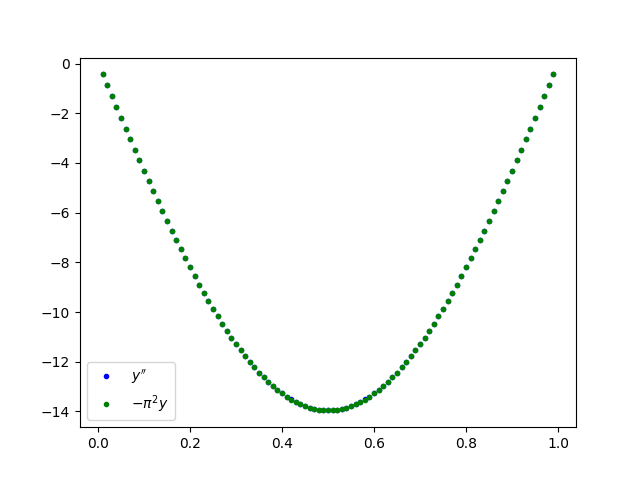
\includegraphics[scale=0.7]{Eigenvectors/Helmholtz.png}
    	\caption{The plot of $y''$ and $-\pi^2y$, apparently they are the same.}
    \end{figure}
    \item (12 points) 
    Use the NumPy function \textit{linalg.eig}() to find the eigenvectors of the Laplacian, 
    print the 3 eigenvalues with the smallest magnitude, 
    and plot the eigenvectors corresponding to them.
    The eigenvalues should be close to $-\pi^{2},-4 \pi^{2}$, and $-9 \pi^{2}$, 
    and the eigenvectors should look like $\psi_{1}, \psi_{2}$, and $\psi_{3}$, as you've shown in Question \ref{q:eigenvector}.
\end{enumerate}

\section{SVD Decomposition (30 points)}

\paragraph{Image Compression} In this question, we will use SVD in the context of image processing. 
To simplify the problem, we focus on the grey-scale image. 
The basic idea is to decomposite the image matrix using SVD and discard those components with small magnitudes.
With only the large components, the image can be saved in lower cost and recovered without losing too much detail.

Let $A$ be any $m \times n$ image matrix. 
Each element represents the grey-scale of one pixel in the original image.
A singular value decomposition of $A$ is a factorization of the following form:
$$
A=U \Sigma V^{T}
$$
where

\begin{itemize}
    \item $U$ is an $m \times m$ orthogonal matrix,
    \item $V$ is an $n \times n$ orthogonal matrix,
    \item $\Sigma$ is an $m \times n$ diagonal matrix.
\end{itemize}

Moreover, it is assumed that diagonal entries of $\Sigma$ are non-negative and we have $\Sigma_{i i}=\sigma_{i}$ with
$$
\sigma_{1} \geq \sigma_{2} \geq \sigma_{3} \geq \cdots \geq \sigma_{p} \geq 0
$$
where $p=\min (m, n)$. 
We call $\sigma_{i}$ singular values of $A$. 
Let $r \leq p$ be the number of non-zero singular values of $A$. 
Then, $\text{rank}(A) = r$.

Then, the non-zero $m \times n$ matrix $A$ of rank $r$ can be constructed from its singular values $\left\{\sigma_{1}, \ldots, \sigma_{r}\right\}$, left singular vectors $\left\{\mathbf{u}_{1}, \ldots, \mathbf{u}_{r}\right\}$, and right singular vectors $\left\{\mathbf{v}_{1}, \ldots, \mathbf{v}_{r}\right\}$ as
$$
A=\sum_{i=1}^{r} \sigma_{i} \mathbf{u}_{i} \mathbf{v}_{i}^{T}
$$

Further, we can approximate $A$ with only a part of singular values and singular vectors. For $k \leq r$, denote $A_{k}$ by
$$
A_{k}:=\sum_{i=1}^{k} \sigma_{i} \mathbf{u}_{i} \mathbf{v}_{i}^{T}
$$
Note that when $\sigma_{i}$ is very small, the term $\sigma_{i} \mathbf{u}_{i} \mathbf{v}_{i}^{T}$ in the above sum becomes negligible. Moreover, since singular values of $A$ are in descending order (stored as diagonal entries of $\Sigma$ in $\left.A=U \Sigma V^{T}\right)$, once $\sigma_{k}$ becomes sufficiently small, we can stop at that value of $k$ and use $A_{k}$ as a reasonable approximation to $A$. 

\begin{enumerate}[label=3.\arabic*]
% \setcounter{enumi}{2}
    \item (10 points) 
    Load the sample image in Appendix \ref{app:sample_img} using Python Imaging Library (See details in Appendix \ref{app:pil}). Compute the singular value decomposition of $A$ using NumPy API \textit{linalg.svd}().
    \item (10 points)
    For $k=2,4,8,16,32,64,128,p$, construct $A_k$ and display the corresponding (approximate) image; you will need to report the rank $k$ in the title of the corresponding figure. Organize your images in a $4\times2$ grid in document.
    \item (10 points)
    Make a plot of singular values of $A$ to see how the size of singular values drop at those point (this gives you an idea of for what $k$, $A_k$ is a reasonably close approximation to $A$).
\end{enumerate}

%%%%%%%%%%%%%%%%%%%%
\section{Nonlinear System (30 points)}
Implement the Newton's method and Secant method to find the roots of the following polynomial:

$$
p(x)=x^{5}-\frac{29 x^{4}}{20}+\frac{29 x^{3}}{36}-\frac{31 x^{2}}{144}+\frac{x}{36}-\frac{1}{720}
$$

on the interval $x \in[0,1]$. 
You must implement Newton's method and Secant method in Python by yourself. 
(Calling the existing functions in package is not allowed.)

\begin{enumerate}[label=4.\arabic*]
    \item (10 points)
    Make a plot of the polynomial on the interval $[0,1]$. How many unique roots are there? 
    \item (10 points)
    Search the root using Newton's method with the initial guess $x_0=0.45$. What is the root of the polynomial at least 10 digits of accuracy?
    \item (10 points)
    Search the root using Secant method with the initial guess $x_0=0.45$ and $x_{-1}=0$. What is the root at least 10 digits of accuracy? Is it same with the Newton's method?
\end{enumerate}

% \bibliographystyle{plain}
% \bibliography{references}

\newpage
\begin{appendices}

\section{Sample Image}\label{app:sample_img}

\begin{figure}[h]
   
\end{figure}



\section{Read and write image in Python}
\label{app:pil}

\begin{minted}[bgcolor=lightgray]{python}

# import
import numpy as np
import PIL
import PIL.Image

# open image in grey-scale
img = PIL.Image.open("lena.jpg").convert('L')
img_seq = img.getdata()
# reshape and normalize to [0,1]
img_arr = np.array(img_seq).reshape(256,256)*(1.0/255)

# do sth...

# new_arr is a 256x256 matrix with the values in [0,1]
y=np.asarray(new_arr*255,dtype=np.uint8)
w=PIL.Image.fromarray(y,mode='L')
w.save("out.png")

\end{minted}


\end{appendices}

\end{document}
